\chapter{ಮೌಸ್ ಬಳಕೆ}
\begin{center}
\begin{figure}[h]
%[trim={left bottom right top},clip]
\begin{tikzpicture}
\node(png){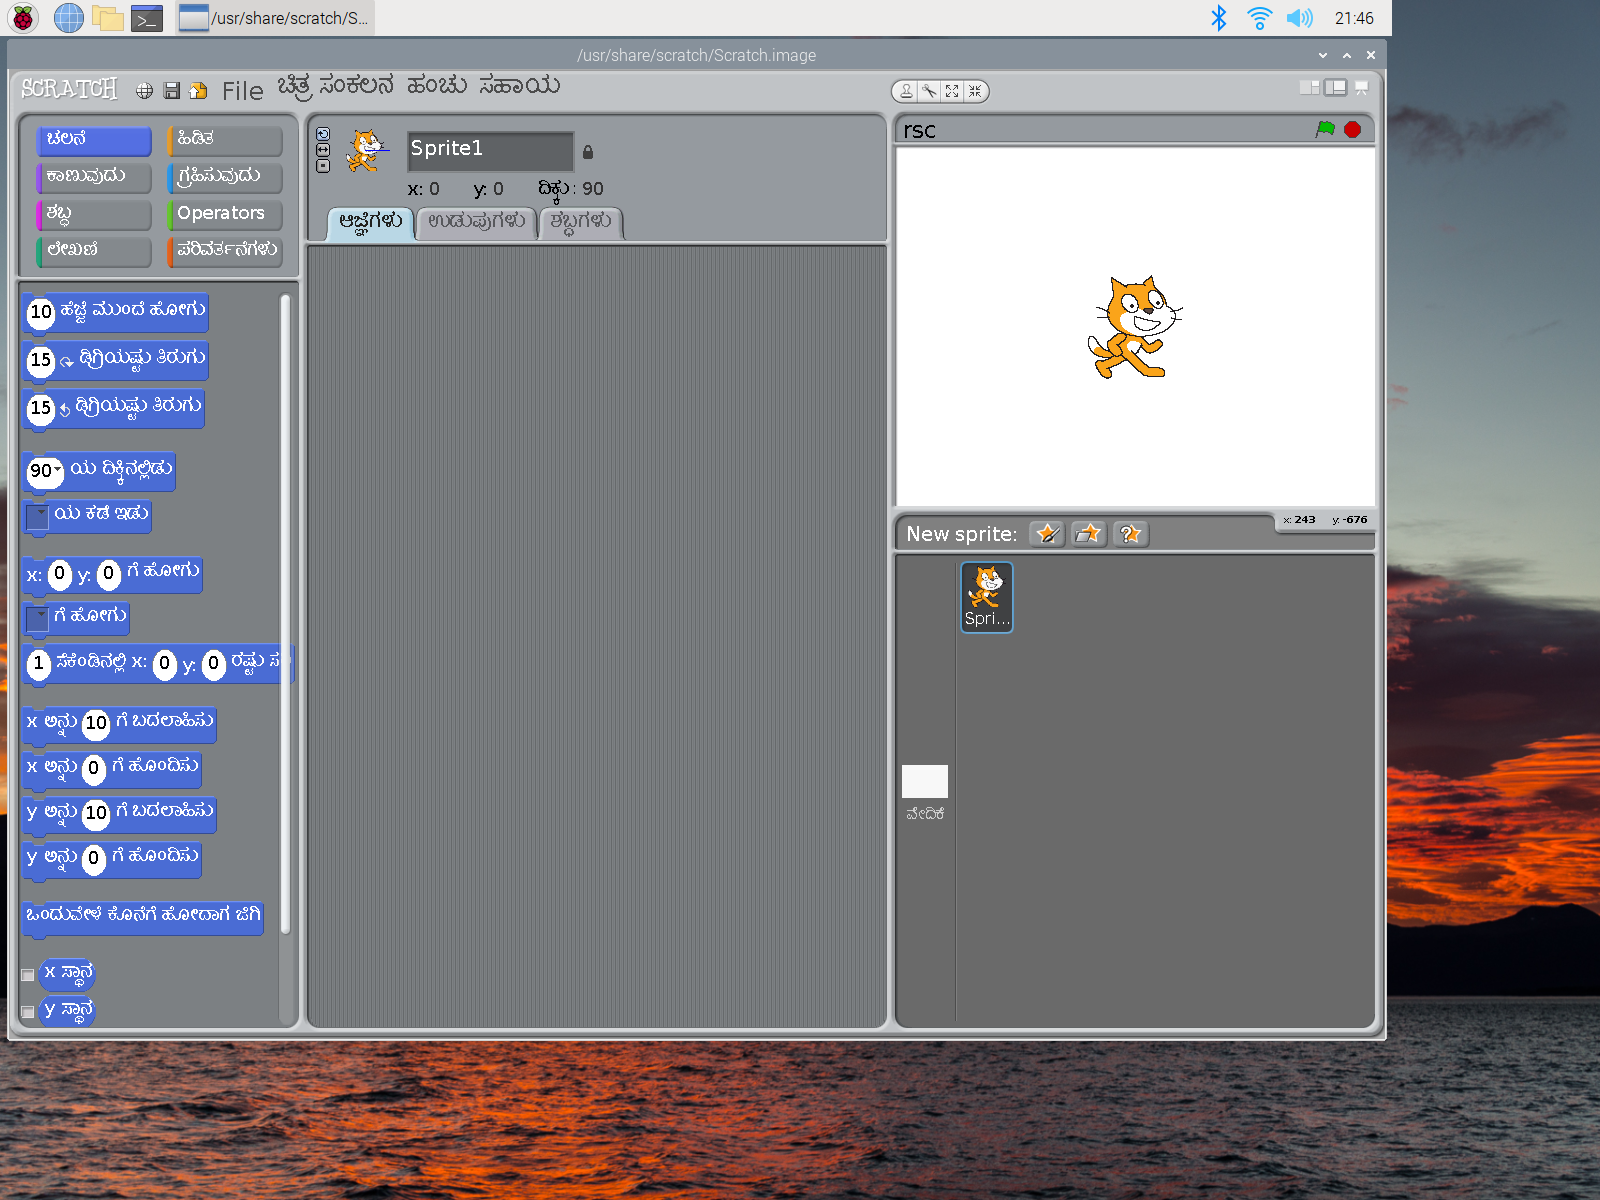
\includegraphics[scale=0.4]{ScratchScreen.pdf}};
\node at (4.4cm,2.2cm)(sprite_main){\Scratchy[0.11]};
\node at (-3.5cm,4.1cm)(sprite_top){\Scratchy[0.05]};
\node at (3cm,-0.5cm)(sprite_btm){\Scratchy[0.04]};
\node at (-6cm,5.5cm)(grp){ ಆಜ್ಞೆಗಳ ಗುಂಪುಗಳು};
\node at (-6cm,-5.6cm)(cmd){ ಚಲನೆ ಗುಂಪಿನ ಆಜ್ಞೆಗಳು};
\node at (-1cm,0)(scratch){ ಪ್ರೋಗ್ರಾಂ ತಯಾರಿಯ ಸ್ಥಳ};
\node at (4.4cm,1cm)(canvas){ ವೇದಿಕೆ};
\draw[->](cmd.north)--++(0.3cm,0.8cm);
\draw[->](grp.south)--++(0.3cm,-1cm);
\end{tikzpicture}
\caption{ಸ್ಕ್ರಾಚ್ ಸ್ಕ್ರೀನ್ ಹೀಗೆ ಕಾಣುತ್ತದೆ}
\label{ScratchScreen}
\end{figure}
\end{center}

ಸ್ಕ್ರಾಚ್ ಪ್ರಾರಂಭಿಸಿದಾಗ ಚಿತ್ರ \ref{ScratchScreen} ನಲ್ಲಿನಂತೆ ಕಾಣಿಸುತ್ತದೆ. ಕಂಪ್ಯೂಟರ್, ನಾವು ನೀಡುವ ಆಜ್ಞೆಗಳಂತೆ ಕೆಲಸ ಮಾಡುತ್ತದೆ.  ಸ್ಕ್ರಾಚ್ನಲ್ಲಿ ಕಂಪ್ಯೂಟರ್ಗೆ ನೀಡುವ ಆಜ್ಞೆಗಳನ್ನು ಮಾಡಿ ತೋರಿಸುವುದಕ್ಕೆ ಒಂದು ಬೆಕ್ಕು ಇದೆ. ಈ ಬೆಕ್ಕಿನ ಹೆಸರು ಸ್ಪ್ರಯ್ಟ್ ಎಂದು. ಸ್ಕ್ರಾಚ್ನಲ್ಲಿ ಸ್ಪ್ರಯ್ಟ್ಗೆ ನೀಡಬಹುದಾದ ಎಲ್ಲಾ ಆಜ್ಞೆಗಳನ್ನು ಎಂಟು ಗುಂಪುಗಳಲ್ಲಿ ವಿಂಗಡಿಸಲಾಗಿದೆ.  ಆಜ್ಞೆಗಳ ಗುಂಪು ಎಲ್ಲಿದೆ ಎಂದು ಚಿತ್ರದಲ್ಲಿ ಕಾಣಿರಿ. ಸಧ್ಯಕ್ಕೆ "ಚಲನೆ" ಮತ್ತು "ಹಿಡಿತ" ಎಂಬ ಎರಡು ಗುಂಪುಗಳಲ್ಲಿನ  ಆಜ್ಞೆಗಳನ್ನು ಬಳಸಿ ಪ್ರೋಗ್ರಾಂ ಬರೆಯುವುದನ್ನು ಕಲಿಯೋಣ.
\section{ಆರಂಭ}

ಮೊದಲಿಗೆ ನೀಲಿ ಬಣ್ಣದ "ಚಲನೆ" ಆಜ್ಞೆಗಳ ಗುಂಪನ್ನು ಒತ್ತಿ.  ನೀಲಿ ಬಣ್ಣದ ಚಲನೆ ಆಜ್ಞೆಗಳ ಕಂಡುಬರುತ್ತವೆ.  ಎಲ್ಲಾ ಚಲನೆ ಆಜ್ಞೆಗಳನ್ನು ಒಮ್ಮೆ ಪರಿಶೀಲಿಸಿ. ಈ ಆಜ್ಞೆಗಳನ್ನು  ಉಪಯೋಗೊಸಿಕೊಡು ಸ್ಪ್ರಯ್ಟ್ ಆನು ಹೇಗೆ ಕೆಲಸ ಮಾಡುವಂತೆ ಪ್ರೋಗ್ರಾಂ ಬರೆಯುವುದು ಎಂದು ಯೋಚಿಸಿ.  ಚಲನೆ ಗುಂಪಿನ ನಂತರ ಕೇಸರಿ ಬಣ್ಣದ "ಹಿಡಿತ" ಆಜ್ಞೆಗಳ ಗುಂಪನ್ನು ಒತ್ತಿ.  ಕೇಸರಿ ಬಣ್ಣದ ಹಿಡಿತ ಆಜ್ಞೆಗಳು ಕಂಡುಬರುತ್ತವೆ.  ಇದೇ ರೀತಿ ಬೇರೆ ಬೇರೆ ಗುಂಪನ್ನು ಒತ್ತಿ ಆ ಗುಂಪಿನ ಆಜ್ಞೆಗಳನ್ನು ಪರಿಶೀಲಿಸಿ.

ಪ್ರೋಗ್ರಾಂ ತಯಾರಿಸುವುದೆಂದರೆ ಈ ಹಲವು ಬಗೆಗಿನ ಆಜ್ಞೆಗಳನ್ನು ಒಂದಾದ ನಂತರ ಒಂದಂತೆ ಜೋಡಿಸಿ ನಮಗೆ ಬೇಕಾದ ಕೆಲಸ ಮಾಡಿಸಿಕೊಳ್ಳುವುದು. ಪ್ರೋಗ್ರಾಂ ತಯಾರಿಯ ಸ್ಥಳದಲ್ಲಿ ಆಜ್ಞೆಗಳನ್ನು ಜೋಡಿಸಿ ಪ್ರೋಗ್ರಾಂ ತಯಾರಿಸಬೇಕು. ಪ್ರೋಗ್ರಾಂನಲ್ಲಿ ನೀಡಿದ ಆಜ್ಞೆಯ ಪ್ರಕಾರ ಸ್ಪ್ರೈಟ್ ಕೆಲಸ ಮಾಡುತ್ತದೆ. ಉದಾಹರಣೆಗೆ “ಹತ್ತು ಹೆಜ್ಜೆ ಮುಂದೆ ಹೋಗು” ಎಂದು ಆಜ್ಞೆ ಮಾಡಿದರೆ ಅದು ಹತ್ತು ಹೆಜ್ಜೆ ಮುಂದೆ ಹೋಗುತ್ತದೆ. ನಂತರ “90 ಡಿಗ್ರಿ ಬಲಕ್ಕೆ ತಿರುಗು” ಎಂದರೆ ಬಲಕ್ಕೆ ತಿರುಗುತ್ತದೆ. ಇನ್ನೂ ಹಲವಾರು ವಿಧದ ಆಜ್ಞೆಗಳನ್ನೆಲ್ಲ ಮುಂದಕ್ಕೆ ಒಂದೊಂದಾಗಿ ತಿಳಿಯೋಣ.

\section{ಆಜ್ಞೆಗಳನ್ನು ಜೋಡಿಸುವುದು}
ಈಗ ಕೆಳಗಿನ ಸೂಚನೆಯಂತೆ ಮೌಸ್ ಉಪಯೊಗಿಸಿ ಮಾಡಿ ನೋಡಿ.  

\begin{enumerate}
\item{"ಚಲನೆ" ಗುಂಪನ್ನು ಒತ್ತಿ.}
\item{"ಚಲನೆ" ಗುಂಪಿನ ಆಜ್ಞೆಗಳನ್ನು ಒತ್ತಿ.}
\item{"ಚಲನೆ" ಗುಂಪಿನ ಆಜ್ಞೆಗಳಲ್ಲಿ ಒಂದನ್ನು ಪ್ರೋಗ್ರಾಂ ತಯಾರಿಯ ಸ್ಥಳದಲ್ಲಿ ತಂದಿರಿಸಿ.}
\item{ಪ್ರೋಗ್ರಾಂ ತಯಾರಿಯ ಸ್ಥಳದಲ್ಲಿರುವ ಆಜ್ಞೆಯನ್ನು ಅತ್ತಿತ್ತ ಜರುಗಿಸಿ.}
\item{ಪ್ರೋಗ್ರಾಂ ತಯಾರಿಯ ಸ್ಥಳದಲ್ಲಿರುವ ಆಜ್ಞೆಗೆ ಮತ್ತೊಂದು ಆಜ್ಞೆಯನ್ನು ಜೋಡಿಸಿ.}
\end{enumerate}

ಜೋಡಿಸುವಾಗ ಎರಡು ಆಜ್ಞೆಗಳು ಹತ್ತಿರ ಬರುತ್ತಿದಂತೆ ಒಂದು ಬಿಳಿ ಗೆರೆ ಕಣಿಸಿಕೊಳ್ಳುವುದನ್ನು ಗಮನಿಸಿ.  ಬಿಳಿ ಗೆರೆ ಕಂಡೊಡನೆ ಒತ್ತಿಟ್ಟುಕೊಂಡ ಮೌಸ್ ಬಿಟ್ಟರೆ ಆಜ್ಞೆಗಳು ಒಂದಕ್ಕೊಂದು ಜೋಡಿಸಿಕೊಳ್ಳುತ್ತವೆ.  ಜೋಡಿ ಆಜ್ಞೆಗಳನ್ನು ಅತ್ತಿತ್ತ ಜರುಗಿಸುವುದಕ್ಕೆ ಮೌಸ್  ಅನ್ನು ಎಲ್ಲಿ ಒತ್ತಿಟ್ಟುಕೊಂಡು ಜರುಗಿಸುತ್ತೇವೆ ಎಂಬುದಕ್ಕೆ ಗಮನ ಕೊಡಬೇಕು. ಜೋಡಿ ಆಜ್ಞೆಗಳಲ್ಲಿ ಮೇಲಿನ ಆಜ್ಞೆಯನ್ನು ಹಿಡಿದು ಅತ್ತಿತ್ತ ಜರುಗಿಸಿದರೆ ಒಟ್ಟು ಪ್ರೋಗ್ರಾಂ ಜರುಗುತ್ತದೆ.

\section{ಆಜ್ಞೆಗಳನ್ನು ಬಿಡಿಸುವುದು}
ಕಂಪ್ಯೂಟರ್ ಪ್ರೋಗ್ರಾಂ ತಯಾರಿಸುವಾಗ ತಪ್ಪುಗಳಾಗುವುದು ಬಹಳ ಸಹಜ. ಹಾಗೆ ತಪ್ಪಾದಾಗ ಅದನ್ನು ತಿದ್ದುವುದು ಹೇಗೆ? ಜೋಡಿ ಆಜ್ಞೆಗಳಲ್ಲಿ ಮೇಲಿನ ಆಜ್ಞೆಯನ್ನು ಹಿಡಿದು ಅತ್ತಿತ್ತ ಜರುಗಿಸಿದರೆ ಒಟ್ಟು ಪ್ರೋಗ್ರಾಂ ಜರುಗುತ್ತದೆ.ಆದರೆ ಕೆಳಗಿನ ಆಜ್ಞೆಯನ್ನು ಹಿಡಿದು ಜರುಗಿಸಿದರೆ ಅದು ಗುಂಪನ್ನು ಬಿಟ್ಟು ಬರುತ್ತದೆ. ಹೀಗೆ ತಪ್ಪಾದ ಆಜ್ಞೆಯನ್ನು ಹೊರತೆಗೆದು ಮತ್ತೆ ಆಜ್ಞೆಗಳ ಗುಂಪಿನಲ್ಲಿ ಬಿಟ್ಟರೆ ಅದು ಮಾಯವಾಗಿ ನಮಗೆ ಪ್ರೋಗ್ರಾಂ ತಿದ್ದಲು ಅವಕಾಶ ಸಿಗುತ್ತದೆ.  ಈಗ ಜೋಡಿಸಿದ  ಆಜ್ಞೆಗಳನ್ನು ಬಿಡಿಸಿ ನೋಡಿ.

\section{ಅಭ್ಯಾಸ}

\begin{figure}[h]
\begin{center}
\begin{Scratch}[1]
\scbox{\cb[w]{10}  ಹೆಜ್ಜೆ ಮುಂದೆ ಹೋಗು}{motion}
\scbox{\cb[w]{20}  ಹೆಜ್ಜೆ ಮುಂದೆ ಹೋಗು}{motion}
\scbox{\cb[w]{30}  ಹೆಜ್ಜೆ ಮುಂದೆ ಹೋಗು}{motion}
\scbox{\cb[w]{40}  ಹೆಜ್ಜೆ ಮುಂದೆ ಹೋಗು}{motion}
\scbox{\cb[w]{50}  ಹೆಜ್ಜೆ ಮುಂದೆ ಹೋಗು}{motion}
\scbox{\cb[w]{100}  ಹೆಜ್ಜೆ ಮುಂದೆ ಹೋಗು}{motion}
\end{Scratch}
\caption{ಮೌಸ್ ಬಳಸುವುದನ್ನು ಅಭ್ಯಾಸ ಮಾಡಲು ಹೀಗೆ ಜೋಡಿಸಿ ಮತ್ತು ಬಿಡಿಸಿ ನೋಡಿ}
\label{mouse1}
\end{center}
\end{figure}

\vspace{-0.5cm}
ಚಿತ್ರ \ref{mouse1} ನಲ್ಲಿನಂತೆ ಆಜ್ಞೆಗಳನ್ನು ಜೋಡಿಸಿ ಮತ್ತು ಬಿಡಿಸಿ ನೋಡಿ.  ಈ ಪ್ರೋಗ್ರಾಂನಂತೆ ಸ್ಪ್ರೈಟ್ ಕೆಲಸ ಮಾಡಿದರೆ ಒಟ್ಟು ಎಷ್ಟು ಹೆಜ್ಜೆ ಮುಂದೆ ಹೋಗಬಹುದು ಎಂದು ಒಮ್ಮೆ ಯೊಚಿಸಿ.

\begin{figure}[h]
\begin{center}
\begin{Scratch}[1]
\boucle{\cb[w]{1} ಮರುಕಳಿಸು}{1}{1}
\scbox{\cb[w]{10}  ಹೆಜ್ಜೆ ಮುಂದೆ ಹೋಗು}{motion}
\end{Scratch}
\caption{ಮರುಕಳಿಸು ಆಜ್ಞೆಯ ಒಳಗೆ ಚಲನೆ ಗುಂಪಿನ ಆಜ್ಞೆಗಳನ್ನು ಜೋಡಿಸಿ ಮತ್ತು ಬಿಡಿಸಿ}
\label{mouse2}
\end{center}
\end{figure}

ಚಿತ್ರ \ref{mouse2} ನಲ್ಲಿನಂತೆ  ಹಿಡಿತ ಗುಂಪಿನಿಂದ ಮರುಕಳಿಸು ಎಂಬ ಆಜ್ಞೆಯನ್ನು ತಂದು ಅದರೊಳಗೆ ಚಲನೆ ಗುಂಪಿನ ಆಜ್ಞೆಯನ್ನು ಜೋಡಿಸಿ.  ಇದೇ ರೀತಿ ಇನ್ನೂ ಹಲವು ಚಲನೆ ಗುಂಪಿನ ಆಜ್ಞೆಗಳನ್ನು ತಂದು  ಜೋಡಿಸಿ ನೋಡಿ. ಈ ಬಾರಿಯೂ,  ಜೋಡಿಸುವಾಗ ಎರಡು ಆಜ್ಞೆಗಳು ಹತ್ತಿರ ಬರುತ್ತಿದಂತೆ ಒಂದು ಬಿಳಿ ಗೆರೆ ಕಣಿಸಿಕೊಳ್ಳುವುದನ್ನು ಗಮನಿಸಿ.  ಬಿಳಿ ಗೆರೆ ಕಂಡೊಡನೆ ಒತ್ತಿಟ್ಟುಕೊಂಡ ಮೌಸ್ ಬಿಟ್ಟರೆ ಆಜ್ಞೆಗಳು ಜೋಡಿಸಿಕೊಳ್ಳುತ್ತವೆ.  ಈಗ ಮರುಕಳಿಸು ಆಜ್ಞೆಯ ಒಳಗಿನಿಂದ ಚಲನೆ ಗುಂಪಿನ ಆಜ್ಞೆಗಳನ್ನು ಬಿಡಿಸಿ ನೋಡಿ.  ಬಿಡಿಸದೆ ಒಟ್ಟು ಪ್ರೋಗ್ರಾಂ ಅನ್ನು ಅತ್ತಿತ್ತ ಜರುಗಿಸುವುದು ಹೇಗೆ ಎಂದು ಕಲಿಯಿರಿ. 

ಈಗ ಚಿತ್ರ \ref{mouse1} ನಲ್ಲಿನ ಎಲ್ಲಾ ಆಜ್ಞೆಗಳನ್ನು ಮರುಕಳಿಸು ಆಜ್ಞೆಯ ಒಳಗೆ ಜೋಡಿಸಿ ಮತ್ತು ಒಂದೊಂದಾಗಿ ಬಿಡಿಸುವುದನ್ನು ಪ್ರಯತ್ನಿಸಿ.

ಚಲನೆ ಗುಂಪಿನ ಆಜ್ಞೆಗಳಲ್ಲಿ ಸಂಖ್ಯೆಗಳಿವೆ. ಇವನ್ನು ಬದಲಾಯಿಸಬೇಕಾದರೆ ಆ ಸಂಖ್ಯೆಯ ಮೇಲೆ ಮೌಸ್ನಿಂದ  ಒತ್ತಿ.  ಆಗ ಸಂಖ್ಯೆಯ ಬಿಳಿ ಹಿಂಭಾಗ, ನೀಲಿ ಬಣ್ಣಕ್ಕೆ ತಿರುಗುತ್ತದೆ. ಹೀಗಿದ್ದಾಗ ಕೀಲಿಮಣೆಯಲಿನ  (\textenglish{keyboard}) ಸಂಖ್ಯೆಗಳ್ಳನ್ನು ಒತ್ತಿದರೆ ಆ ಸಂಖ್ಯೆಗಳು, ಆಜ್ಞೆಗೆ ಸೇರಿಕೊಳ್ಳುತ್ತದೆ. ಇದನ್ನೂ ಅಭ್ಯಾಸ ಮಾಡಿ. 

